%!TEX root = ../Thesis.tex
%Chapter 5

\chapter{Heat Rectification in graded chains of trapped ions}
\label{Chapter5}
\lhead{Chapter 5. \emph{Heat Rectification in graded chains of trapped ions}} % Write in your own chapter title to set the page header
%
We numerically demonstrate heat rectification for linear chains of  ions in trap lattices with  graded  trapping frequencies, in contact with
thermal baths implemented by optical molasses.  To calculate the local temperatures and heat currents we find the stationary state
by solving a system of algebraic equations. This approach is much faster than the usual method
that integrates the dynamical equations of the system and averages over noise realizations.
%
\newpage
%
\section{Introduction\label{IntroductionRectificationChainOfIons}}

The ideal thermal rectifier, also ``thermal diode'',  is a device that allows heat to propagate in one direction, from a hot to a cold bath, but not in the opposite one when the temperature bias of the baths is  reversed. The name is set by analogy to the
half-wave rectifiers or diodes for electric current. More generally thermal rectification simply denotes
asymmetric heat flows (not necessarily all or nothing) when the bath temperatures are reversed.
 Thermal rectification was discovered by C. Starr in 1936 in a junction between copper and cuprous oxide \cite{Starr1936}. Many years later, a work of Terraneo \textit{et al.} demonstrated thermal rectification in a model
consisting on a segmented chain of coupled nonlinear oscillators  in contact with two thermal baths at temperatures $T_H$ and $T_C$, with $T_H > T_C$ \cite{Terraneo2002}. This paper sparked a substantial body of research  that spans to this day \cite{Pereira2019} (see Fig. 1 in \cite{Roberts2011}).

\begin{figure*}
    \centering
    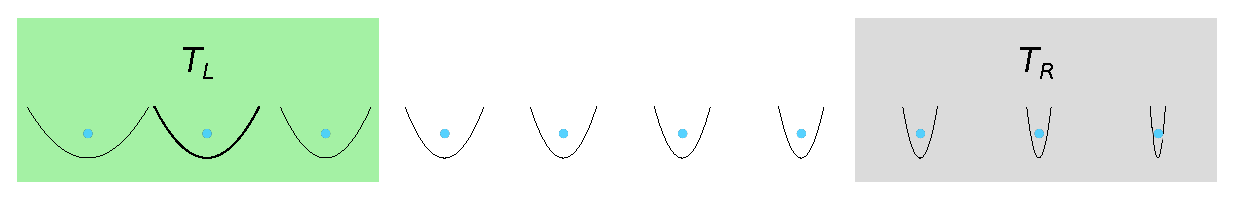
\includegraphics[width=0.9\linewidth]{Figures/Diagram.eps}
    \caption{Schematic representation  of the frequency-graded chain of trapped ions proposed as a thermal rectifier. The left and right ends of the chain are in contact with optical molasses at temperatures $T_L$ and $T_R$ (green and grey boxes respectively). Each ion is in an individual trap. The (angular) frequencies of the traps increase homogeneously from left to right, starting from $\omega_1$ and ending at $\omega_1+\Delta\omega$. The ions interact through the Coulomb force, which is long range, and therefore all the ions interact among them, even distant neighbors. By default  we use 15 ions.}
    \label{fig:Diagram}
\end{figure*}

Research on thermal rectification has gained a lot of attention in recent years as a key ingredient to build
prospective devices to control heat flows similarly to electrical currents \cite{Roberts2011,Li2012}. There are  proposals
%that exploit the analogy with electronic currents
to engineer thermal logic circuits \cite{Ye2017} in which information, stored in thermal memories \cite{Wang2008}, would be processed in thermal gates \cite{Wang2007}. Such thermal gates, as their electronic counterparts,  will require thermal diodes and thermal transistors  to operate \cite{Li2006,Joulain2016}.
%Information may also be stored in thermal memories \cite{Wang2008}.
Heat rectifying devices would also be quite useful  in nano electronic circuits, letting delicate components dissipate heat while being protected from external heat sources \cite{Roberts2011}.

Most work on thermal diodes has been theoretical with only a few experiments \cite{Chang2006,Kobayashi2009,Leitner2013,Elzouka2017}.
A relevant attempt to build a thermal rectifier was based on a graded structure made of carbon and boron nitride nanotubes that transports heat between a pair of heating/sensing circuits \cite{Chang2006}. One of the ends of the nanotube is loaded with a deposition of another material, which makes the heat flow better from the loaded end to the unloaded end. However, rectifications were small, with rectification factors (relative
heat-flow differentials) around $7\%$.
% in \cite{Chang2006}).

Much effort has been aimed at improving the rectification factors and the features of the rectifiers. Some works
relied, as in \cite{Terraneo2002}, on a chain segmented into two or more regions  with different properties,  but using other lattice models such as the Frenkel-Kontorova (FK) model \cite{Li2008,Hu2006}.
The fundamental ingredient for having rectification  was attributed to nonlinear forces in the chain \cite{Zeng2008,Katz2016,Li2008,Hu2006,Benenti2016,Li2012}, which lead to a temperature dependence of the phonon bands or power spectral densities. The bands may match or mismatch at the
interfaces depending on the sign of the temperature bias of the baths, allowing or obstructing heat flow \cite{Terraneo2002,Li2004}.  Later, alternative mechanisms have been
proposed which do not necessarily rely on anharmonic potentials \cite{Pereira2017,Pons2017}.
Also, Peyrard provided a simple model to explain and build rectifiers based on assuming the Fourier law for heat conduction locally
combined with a temperature and position-dependent conductivity \cite{Peyrard2006}.


It was soon realized that the performance of segmented rectifiers was very sensitive to the size of the device, i.e., rectification decreases with increasing the length of the rectifier \cite{Hu2006}. To overcome this limitation two ideas were proposed. The first one consists in using graded rather than segmented chains, i.e., chains where some physical property varies continuously along the site position such as the mass of particles in the lattice \cite{Wang2012,Chen2015,Romero-Bastida2017,Yang2007,Romero-Bastida2013,Dettori2016,Pereira2010,Pereira2011,Avila2013}. The second one uses particles with long-range interactions (LRI), such that all the particles in the lattice interact with each other \cite{Chen2015,Bagchi2017,Pereira2013}. The rationale behind was that in a graded system new asymmetric, rectifying channels are created, while the long-range interactions create
also new transport channels, avoiding the usual decay of heat flow with size \cite{Chen2015}.
%
% ``\textit{with long-range interactions (LRI), we conjecture that the presence of new links (interactions) among different sites creates new channels for the heat transport... Besides that, in a graded system... new asymmetric channels are created which in turn favors the asymmetric flow, i.e., rectification}'' \cite{0295-5075-111-3-30004}.
%
Besides a stronger rectification power, LRI graded chains are expected to have better heat conductivity than segmented ones. This is an important point for technological applications, because devices with high rectification factors are not useful if the currents that flow through them are very small.

In this article we propose to bridge the gap between mathematical models and actual systems
exploring the implementation of a heat rectifier in a realistic, graded system with long-range interactions:
a chain of  ultracold ions in a segmented Paul trap with graded microtraps for each ion.
Long-range interactions are due to the Coulomb forces, and the  baths at the ends of the chain  may be implemented with optical molasses,
see Fig. \ref{fig:Diagram}. The trapping frequencies of the  microtraps are controlled individually in order to create a graded and asymmetric trap-frequency profile along the chain. This asymmetry will lead to a heat flow that depends on the sign of the temperature difference of the baths. Heat transport in trapped ion chains has been studied in several works  \cite{Freitas2015,Ruiz2014,Ruiz2019,Pruttivarasin2011,Ramm2014} and interesting phenomena like phase transitions have been investigated \cite{Freitas2015,Ruiz2014,Ruiz2019,Pruttivarasin2011}. The idea of using locally-controlled traps is already mentioned in \cite{Freitas2015} to implement disorder and study its effects. The device we present here may be challenging to implement, but at reach with the current technology, in particular  that of microfabricated traps \cite{Cirac2000,Krauth2014,Schmied2009}. Thus the setting is thought for a small, realistic number of controllable ions.
% and, while refraining from scaling up the size of the chain beyond realistic
%values, we shall nevertheless analyze  the dependence with the number of ions.

The rest of the article is organized as follows. In Section \ref{Physical System} we describe the physical system of trapped ions with graded trap frequencies. We also set the stochastic dynamics due to the action of lasers at the chain edges.
In Section \ref{sec:HeatFlow}  we implement an efficient  method to find the steady state using Novikov's theorem and solving an algebraic system of equations. In Section \ref{Numerical Results} we present simulations of this system exhibiting thermal rectification and discuss the dependence with ion number, different options for the ion-laser coupling, and the advantages/disadvantages of using a graded frequency profile instead of a segmented one. Finally, in Section \ref{ConclusionsRectificationChainOfIons} we summarize our conclusions, and discuss connections with other works.
%
%
%
\section{Physical System\label{Physical System}}
%
%
%
%
Consider a linear lattice of $N$ individual harmonic traps of (angular) trapping frequencies  $\omega_n$ evenly distributed along the $x$ axis at a distance $a$ from each other. Each trap contains a single ion that interacts with the rest via Coulomb potentials. All the ions are of the same species, with mass $m$ and charge $q$. The Hamiltonian that describes the dynamics of the system is (we consider only linear, one dimensional motion along the chain axis)
%
\begin{equation}
    H(\bm{x},\bm{p}) = \sum_{n=1}^N \left[\frac{p_n^2}{2m}  + \frac{m\omega_n^2}{2} (x_n - x_n^{(0)})^2\right] + V_{int}(\bm{x}),
    \label{eq:ChainHamiltonian}
\end{equation}
%
where $\{x_n,p_n\}$, position and momentum of each ion, are the components of  the vectors
$\bm{x},\bm{p}$, $x_n^{(0)} = n  a$ are the centers of the harmonic traps, and $V_{int}$ is the sum of the Coulomb interaction potential between all  pairs of ions,
%
\begin{equation}
    V_{int}(\bm{x}) = \frac{1}{2}\sum_n \sum_{l\neq n} V_{C}(\left|x_n-x_l\right|),
    \label{eq:InteractionHamiltonian}
\end{equation}
%
with $V_{C}(\left|x_n-x_l\right|) = \frac{q^2}{4\pi\varepsilon_0}\frac{1}{\left|x_n-x_l\right|}$. The ends of the chain are in contact with two thermal reservoirs at temperatures $T_L$ for the left bath and $T_R$ for the right bath respectively. The action of the resevoirs on the dynamics of the chain is modeled via Langevin baths at temperatures $T_L$ and $T_R$ \cite{Lepri2003,Dhar2018}. The equations of motion of the chain, taking into account the baths and the Hamiltonian, are
%
\begin{equation}
    \begin{split}
        \dot{x}_n &= \frac{1}{m}p_n, \\
        \dot{p}_n &= - m\omega_n^2 (x_n-x_n^{(0)}) - \frac{\partial V_{int}}{\partial x_n} - \frac{\gamma_n}{m}p_n + \xi_n(t),
    \end{split}
    \label{eq:Dynamics}
\end{equation}
%
where $\gamma_n$ and $\xi_n(t)$ are only non-zero for the ions in the end regions, in contact with the left and right baths in the sets ${\cal L} = \left\{1,2,...,N_L\right\}$ and \linebreak ${\cal R} = \left\{N-(N_R-1),...,N-1,N\right\}$,  see Fig. \ref{fig:Diagram}. The $\gamma_n$ are friction coefficients and $\xi_n(t)$ are uncorrelated Gaussian noise forces satisfying $\expval{ \xi_n(t)} = 0$ and $\expval{ \xi_n(t)\xi_m(t') } = 2 D_n \delta_{nm}\delta(t-t')$, $D_n$ being the diffusion coefficients. These Gaussian forces are formally the time derivatives of independent Wiener processes (Brownian motions)   $\xi_n(t) = \sqrt{2D_n}\frac{dW_n}{dt}$ \cite{Toral2014,Ruiz2014} and Eq. \eqref{eq:Dynamics} is a stochastic differential equation (SDE) in the Stratonovich sense \cite{Toral2014}.

The baths are physically implemented by optical molasses consisting of a pair of counterpropagating Doppler-cooling lasers \cite{Ruiz2014}. The friction and diffusion coefficients for the ions in contact with the baths are given by \cite{Cohen1992,Metcalf2003,Ruiz2014}
%
\begin{equation}
    \begin{split}
        \gamma_n &= -4 \hbar k_{L,R}^2 \left(\frac{I_{L,R}}{I_0}\right)\frac{2\delta_{L,R}/\Gamma}{\left[1 + (2\delta_{L,R}/\Gamma)^2\right]^2},\\
        %
        D_n &= \hbar^2 k_{L,R}^2 \left(\frac{I_{L,R}}{I_0}\right) \frac{\Gamma}{1 + (2\delta_{L,R}/\Gamma)^2},\\
        n &\in \cal{L},\cal{R},
    \end{split}
    \label{eq:DopplerCooling}
\end{equation}
%
where $k_L$ ($k_R$) and $I_L$ ($I_R$) are the wave vector and intensity of the left (right) laser. $\delta_L$ ($\delta_R$) is the detuning of the left (right) laser with respect to the angular frequency $\omega_0$ of the atomic transition the laser is exciting, and $\Gamma$ is the corresponding natural line width of the  excited state. The expressions in Eq. \eqref{eq:DopplerCooling} are valid only if the intensities of the lasers are small compared to the saturation intensity $I_0$, $I_{L,R}/I_0\ll 1$. In this bath model, the friction term in Eq. \eqref{eq:Dynamics} comes from the cooling action of the laser and the white noise force $\xi_n(t)$ corresponds to the random recoil of the ions due to spontaneous emission of photons \cite{Metcalf2003,Cohen1992}. Using the diffusion-dissipation relation $D = \gamma k_B T $ \cite{Chee2010}, the temperatures of the optical molasses baths are given by
%
\begin{equation}
    T_{L,R} = -\frac{\hbar \Gamma}{4 k_B} \frac{1+(2\delta_{L,R}/\Gamma)^2}{(2\delta_{L,R}/\Gamma)},
    \label{eq:Doppler}
\end{equation}
%
with $k_B$ being the Boltzmann constant. If the laser intensities are low enough, the temperatures of the baths are controlled by modifying the detunings. When $\delta = \delta_D=-\Gamma / 2$ the optical molasses reach their minimum temperature possible, the Doppler limit $T_{D} = {\hbar \Gamma}/({2k_B})$. Note that away from the Doppler limit the same temperature may be achieved
for two different values of detuning. These two possibilities imply different couplings (two different pairs of $\gamma$ and $D$ values) and thus different physical effects that will be studied in Sec. \ref{TC}.
%
%
%
%
\section{Calculation of the stationary heat currents\label{sec:HeatFlow}}
%
%
The local energy of each site is defined by
%
\begin{equation}
    H_n = \frac{1}{2m} p_n^2 + \frac{1}{2}m\omega_n^2 \left( x_n - x_n^{(0)}\right)^2 +\frac{1}{2}\sum_{l\neq n} V_C(\left|x_n-x_l\right|).
    \label{eq:LocalEnergy}
\end{equation}
%
Differentiating $H_n$ with respect to time we find the continuity  equation
%
\begin{equation}
    \dot{H}_n = \frac{p_n}{m}\! \left[ \xi_n(t)-\gamma_n \frac{p_n}{m} \right]\! - \frac{1}{2m}\!\sum_{l\neq n}\frac{\partial V_C (\left|x_n\!-\!x_l\right|)}{\partial x_n}(p_n + p_l).
    \label{eq:continuityFirst}
\end{equation}
%
Two different contributions can be distinguished: $j^B_n \equiv \frac{p_n}{m} \left[ \xi_n(t)-\gamma_n \frac{p_n}{m} \right]$, which is the energy flow from the laser reservoir to the ions at the edges of the chain (only for $n\in {\cal L}, {\cal R}$), and $\dot{H}_n^{int} \equiv - \frac{1}{2m}\sum_{l\neq n}\frac{\partial V_C (\left|x_n-x_l\right|)}{\partial x_n}(p_n + p_l)$, which gives the ``internal'' energy flow due to the interactions with the rest of the ions. In the steady state $\expval{\dot{H}_n} = 0$, and therefore
%
\begin{equation}
    \expval{j^B_n} + \expval{\dot{H}_n^{int}} = 0,
    \label{eq:continuitySecond}
\end{equation}
%
where $\langle \cdot\!\cdot\!\cdot \rangle$ stands for the expectation value with respect to  the ensemble of noise processes $\bm\xi (t)$ ($\bm\xi$ represents a vector with
components $\xi_n$). Equation \eqref{eq:continuitySecond} implies that, in the steady state, the internal rates $\dot{H}_n^{int}$ vanish for the inner ions of the chain because $j^B_n = 0$ for $n\notin {\cal L},{\cal R}$. In chains with nearest-neighbor (NN) interactions,
$\langle\dot{H}_n^{int}\rangle$ simplifies to two compensating and equal-in-magnitude contributions that define the homogeneous heat flux across the chain.
For long-range interactions this is not so and defining the flux is not so straightforward. A formal possibility is to impose
nearest-neighbor interatomic interactions for some atoms in the chain \cite{Chen2015},
but this approach is not realistic in the current system so we define instead the heat currents
for the left and right baths as
%
\begin{equation}
    \begin{split}
        J_L (t)&= \sum_{n\in {\cal L}} \expval{j^B_n},\\
        J_R (t)&= \sum_{n\in {\cal R}} \expval{j^B_n},
    \end{split}
    \label{eq:BathHeatFlows}
\end{equation}
%
respectively. These expressions are in general time-dependent.
In the steady state we must have $J_{L,{\rm steady}} + J_{R,{\rm steady}} = 0$, since the local energies stabilize and internal energy
flows cancel. We use either $J_{L,{\rm steady}}$ or $J_{R,{\rm steady}}$ to calculate the total energy flow in the chain, always taking the absolute value, i.e., $J \equiv \abs{J_{L,{\rm steady}}}= \abs{J_{R,{\rm steady}}}$. $J$ is defined as $J_\rightarrow$ when the hot bath is on the left
and $J_\leftarrow$ when it is on the right.

To compute the average heat fluxes of the baths $\expval{j^B_n}$ in Eq. \eqref{eq:BathHeatFlows} we need
the averages $\expval{p_n(t)\xi_n(t)}$. Instead of explicitly averaging $p_n(t)\xi_n(t)$ over different realizations of the white noise we use Novikov's theorem \cite{Novikov1965,Ma2011,Toral2014}. Novikov's theorem states that the ensemble average (over  the realizations of the noise) of the product of some functional $\phi(t)$, which depends on a Gaussian noise $\xi(t)$ with zero mean value, $\expval{\xi(t)} = 0$, and the noise itself, is given by
%
\begin{equation}
    \expval{\xi(t)\phi(t)} = \int_0^t dt' \expval{\xi(t)\xi(t')} \expval{\frac{\delta \phi(t)}{\delta\xi(t')}},
    \label{eq:Novikov_GeneralExpression}
\end{equation}
%
where ${\delta \phi(t)}/{\delta\xi(t')}$ is the functional derivative of $\phi(t)$ with respect to the noise, with $t'<t$. When the noise is $\delta-$correlated, $\expval{\xi(t)\xi(t')}=2D\delta(t-t')$, and Eq. \eqref{eq:Novikov_GeneralExpression} reads $\expval{\xi(t)\phi(t)} = D \expval{{\delta \phi(t)}/{\delta\xi(t')}}|_{t' \to t^-}$. To apply Novikov's theorem to our model we need the functional derivatives of the position $x_n(t)$ and momentum $p_n(t)$ coordinates with respect to the white noises. We integrate Eq. \eqref{eq:Dynamics} to have its formal solution as a functional depending on the white Gaussian noises $\xi_n(t)$,
%
\begin{equation}
    \begin{split}
        x_n(t) &= x_n(0) +  \frac{1}{m}\int_0^t ds\; p_n(s) ,\\
        p_n(t) &= p_n(0) + \int_0^t ds\; \left[ -\frac{\partial H}{\partial x_n}(s) - \frac{\gamma_n}{m}p_n(s) + \xi_n(s)\right].
    \end{split}
    \label{eq:FormalSolution}
\end{equation}
%
Equation \eqref{eq:FormalSolution} implies that the functional derivatives are ${\delta x_n(t)}/{\delta \xi_m(t')}|_{t'\to t^-} = 0$ and
${\delta p_n(t)}/{\delta \xi_m(t')}|_{t'\to t^-} = \delta_{nm}$ ($\delta_{nm}$ is the usual Kronecker delta symbol). Thus we have $\expval{x_n(t) \xi_m(t)} = 0$ and $\expval{p_n(t) \xi_m(t)} = \delta_{nm}D_m$, which gives for the heat flow from the baths
%
\begin{equation}
    \expval{j^B_n} = \frac{1}{m} \left[ D_n-\gamma_n \frac{\expval{p_n^2}}{m} \right].
\end{equation}
%
In all simulations we check that $|J_{L,{\rm steady}}|=|J_{R,{\rm steady}}|$ within the numerical tolerance of the computer. To measure the asymmetry of the heat currents we use the rectification factor $R$ defined as
%
\begin{equation}
    R = \frac{ J_\rightarrow - J_\leftarrow}{max(J_\rightarrow,J_\leftarrow)}.
    \label{eq:R_Factor}
\end{equation}
%
$R$ values may go from $-1$ to $1$ (In the figures we depict it in \% between -100\% and 100\%). If there is no rectification $J_\rightarrow = J_\leftarrow $ and $R=0$. For perfect rectification in the right (left) direction, $J_\rightarrow \gg J_\leftarrow$ ($J_\rightarrow \ll J_\leftarrow$), and $R = 1$ ($R = -1$).
Take note that other  definitions of rectification factors exist in many works
on asymmetric heat transfer so comparisons should be done with care.
%

This model does not show the antithermodynamical behavior  observed in other models
\cite{De-Chiara2018,Levy2014}, and heat is found to flow in all cases from the hot to the
cold bath.
% blue{The Langevin bath is known to be equivalent to a local master equation, which can give thermodynamical inconsistencies . However, we have not observed any violation of the first and second laws of thermodynamics in our simulations, since the system reaches a steady state where the incoming and outcoming heat currents compensate each other and heat always flows from the hot to the cold bath.}%
%
%
%
\subsection{Algebraic, small-oscillations approach to calculate the steady state\label{steadyState}}
%
%
%
%
To find the temperature profiles and heat currents in the steady state the usual approach is to solve the SDE system in Eq. \eqref{eq:Dynamics} up to long times  and for many realizations of the white noises $\bm\xi (t)$. In that way the ensemble averages $\expval{p_n(t \to \infty)^2}$, necessary for both the temperature profiles and heat currents, are computed. This standard route implies a heavy computational effort, in particular  when we want to study the heat transport for several bath configurations, frequency increments and chain parameters. It is possible to circumvent this difficulty and find ensemble averages like $\expval{x_n x_m}$, $\expval{x_n p_m}$, $\expval{p_n p_m}$ (second order moments) without integrating any SDE \cite{Sarkka2019}. The idea is to impose the condition ${d\expval{\cdot\cdot\cdot}}/{dt} = 0$ for all the second order moments and linearize the dynamical equations of the system around equilibrium.
A system of linear algebraic equations for the moments results, that can be easily solved without solving the SDE many times.
% to solve a system of linear algebraic equations. We will analyze the validity of the linearized approximation in the following section.


To linearize the SDE in Eq. \eqref{eq:Dynamics} we approximate the potential energy of the Hamiltonian in Eq. \eqref{eq:ChainHamiltonian}, $V(\bm{x}) = V_{int}(\bm{x}) + m\;\sum_n \omega_n^2 (x_n-x_n^{(0)})^2/2$, by its harmonic approximation around the equilibrium positions $\bm{x}^{eq}$, defined by  $\frac{\partial V(\bm{x})}{\partial\bm{x}}\Big|_{\bm{x}=\bm{x}^{eq}} = 0$. The approximate potential (ignoring the zero-point energy) is
%
\begin{equation}
    V(\bm{x})\approx  \frac{1}{2} \sum_{n,m} K_{nm} (x_n-x_n^{eq})(x_m-x_m^{eq}),
\end{equation}
%
with $K_{nm} = \frac{\partial^2 V(\bm{x})}{\partial x_n \partial x_m}\Big|_{\bm{x}=\bm{x}^{eq}}$ being the Hessian matrix entries of $V(\bm{x})$ around the equilibrium configuration \cite{James1998}
%
\begin{equation}
    K_{nm} =
    \begin{cases}
        m \omega_n^2 + 2 \left(\frac{q^2}{4\pi\varepsilon_0}\right) \sum_{l \neq n  }\frac{1}{\left|x_n^{eq}-x_l^{eq}\right|^3} & \text{if  } n=m\\

         - 2 \left(\frac{q^2}{4\pi\varepsilon_0}\right) \frac{1}{\left|x_n^{eq}-x_m^{eq}\right|^3} & \text{if  } n \neq m
    \end{cases}.
\end{equation}
%
Note that this approximation does not modify the two main features of the system, namely asymmetry and long-range interactions, which are manifest in the asymmetric distribution of $\omega_n$ and the non-zero off-diagonal elements of the $K$ matrix, respectively. In the following we will use $y_n=x_n-x_n^{eq}$ to simplify the notation. The linearized dynamics around the equilibrium positions are given by
%
\begin{equation}
    \begin{split}
        \dot{y}_n &= \frac{1}{m}p_n,\\
        \dot{p}_n &= -\sum_{l}K_{nl}y_l- \frac{\gamma_n}{m}p_n + \xi_n(t).
    \end{split}
    \label{eq:DynamicsHarmonic}
\end{equation}
%
Now, we set ${d\expval{\cdot\!\cdot\!\cdot}}/{dt} = 0$ for all the moments. Using Eq. \eqref{eq:DynamicsHarmonic} and applying Novikov's theorem we find
%
% \begin{widetext}
% \begin{eqnarray}
%     \frac{d}{dt}(x_n x_l) &=& \frac{1}{m}(x_n p_l + x_l p_n) , \nonumber\\
%     \frac{d}{dt}(x_n p_l) &=& \frac{1}{m}\left(p_n p_l - \gamma_l x_n p_l\right) - \sum_m K_{lm}x_n x_m + x_n \xi_l , \nonumber\\
%     \frac{d}{dt}(p_n p_l) &=& - \sum_m x_m\left( K_{nm}p_l + K_{lm} p_n \right) - \frac{1}{m}(\gamma_l + \gamma_n) p_n p_l + \xi_n p_l + \xi_l p_n .
% \label{eq:DynamicsHarmonicOfMomenta}
% \end{eqnarray}
% \end{widetext}
%
% Now we make use of $\frac{d\expval{}}{dt} = 0$ and the Novikov theorem \cite{1965JETP20.1290N,PhysRevB.83.134418}, which in this case implies $\expval{ x_n \xi_l } = 0 $ and $\expval{ p_n \xi_l } = \delta_{nl}D_n$, to finally find
%
\begin{equation}
    \begin{split}
        \expval{p_n p_l} - \gamma_l\expval{y_n p_l} - \sum_m K_{lm}\expval{y_n y_m} &= 0,\\
        \sum_{m}\left[ K_{nm}\expval{y_m p_l} + K_{lm}\expval{y_m p_n} \right] + \frac{1}{m}\left( \gamma_l + \gamma_n \right)\expval{p_n p_l} &= 2 \delta_{nl} D_n.
    \end{split}
    \label{eq:SteadyStateEquation}
\end{equation}
%
The system \eqref{eq:SteadyStateEquation} is linear in the second order moments so it can be solved numerically to find the steady-state values of the moments. Besides Eq. \eqref{eq:SteadyStateEquation} we have that $\expval{y_n p_l} = - \expval{y_l p_n}$, which follows from Eq. \eqref{eq:DynamicsHarmonic} and $d\expval{y_n y_m}/dt = 0$. Since there are $\frac{1}{2}N(N-1)$ independent $\expval{y_n p_l}$ moments, we choose the ones with $n<l$. Similarly, the moments $\expval{y_n y_l}$ and $\expval{p_n p_l}$ contribute with $\frac{1}{2}N(N+1)$ independent variables each and we choose the ones with $n\leq m$. Thus there are in total $\frac{1}{2}N(3N+1)$ independent moments that we arrange in the vector
%
\begin{equation}
\begin{split}
    \bm\eta = \Big[ &\expval{y_1 y_1},\expval{y_1 y_2},...,\expval{y_N y_N},\\
    &\expval{p_1 p_1},\expval{p_1 p_2},...,\expval{p_N p_N},\\
    &\expval{y_1 p_2},\expval{y_1 p_3},...,\expval{y_{N-1} p_N}\Big]^T.
    \label{eq:CovariancesVector}
\end{split}
\end{equation}
%
There are the same number of independent equations
%in Eq. \eqref{eq:SteadyStateEquation}
as independent moments: $N^2$
equations correspond to the first line in Eq.  \eqref{eq:SteadyStateEquation}, and $\frac{1}{2}N(N+1)$ equations
to the second line because of the symmetry with respect to $n,l$. The system of equations \eqref{eq:SteadyStateEquation} may be compactly written as $\mathbf{A}\boldsymbol\eta = \mathbf{B}$, where $\mathbf{A}$ and $\mathbf{B}$ are a $\frac{1}{2}N(3N+1)$ square matrix and vector.
% which are built by rearranging the coefficients in the left and right hand sizes of \eqref{eq:SteadyStateEquation} in the appropiate way.
%
%
%
%
%
\section{Numerical Results\label{Numerical Results}}
%
%
%
%
%
\begin{figure}[h]
    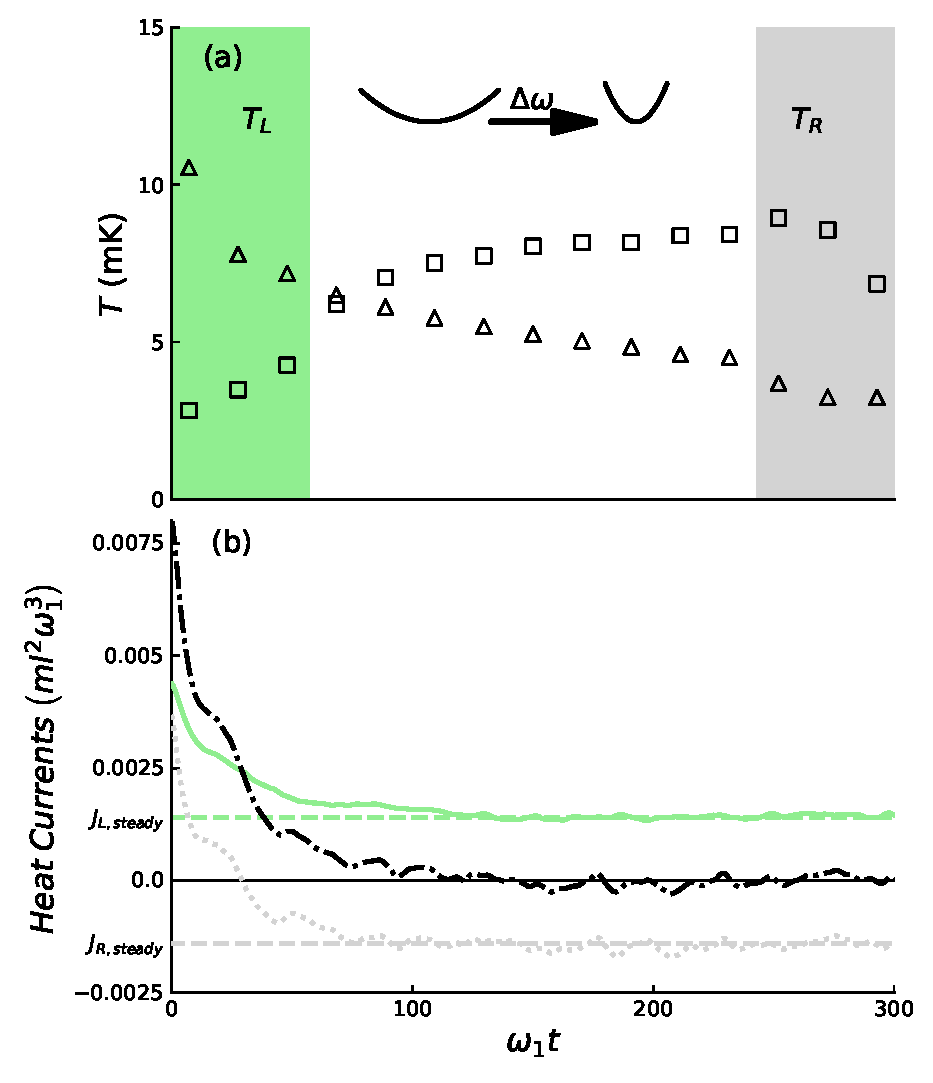
\includegraphics[width=\linewidth]{Figures/24Mg_Temperature_Profiles_And_Evolution.eps}
 \caption{(a) Temperatures of the ions in the stationary state for a graded chain with the parameters described in section \ref{Results_A}. The temperature profiles found with the algebraic method (Eq. \eqref{eq:SteadyStateEquation}) are indistinguishable from the ones found solving the Langevin equation (Eq. \eqref{eq:Dynamics}). Empty triangles (squares) correspond to $T_L = T_H$ ($T_L = T_C$) and $T_R = T_C$ ($T_R = T_H$). (b) Heat currents  as a function of time for $T_L = T_H$ and $T_R = T_C$, see Eq. (\ref{eq:BathHeatFlows}): $J_L(t)$ (solid green line) from the left reservoir into the chain;
 $J_R(t)$ (dotted grey line) from the right reservoir into the chain (negative except at very short times); $J_L(t)+J_R(t)$
 (dotted-dashed black line), which must go to zero in the steady state. The three lines tend to stationary values marked by horizontal lines. Parameters: $\omega_1 = 2\pi \times 50$ kHz,
$a=50\, \mu$m,  $\delta_H = -0.02 \, \Gamma$, and $\delta_C = -0.1 \, \Gamma$, which gives temperatures $T_H \approx 12$ mK and $T_C \approx 3$ mK. $\Delta\omega = 0.5 \, \omega_1$. In all figures $\Gamma = 2\pi \times 41.3$ MHz.}
    \label{fig:Temperature_Profiles_Magnesium}
\end{figure}

We now display the results of our simulations. To find the temperature profiles and the currents in the steady state we use the algebraic method described in section \ref{steadyState}. We also check that the results coincide with those by solving Eq. \eqref{eq:Dynamics} for many different realizations of the noisy forces $\bm\xi (t)$ and averaging. The code for all the numerical simulations has been written in the language \textit{Julia} \cite{Bezanson2012,Bezanson2017}. In particular, to solve the Langevin equation, we used \textit{Julia}'s package \textit{DifferentialEquations.jl} \cite{Rackauckas2017}.

To model the baths and the chain we use atomic data taken from ion trap experiments \cite{Leupold2015,Lo2015}. We consider 15 $^{24}$Mg$^+$ ions in all figures except in Fig. \ref{fig:N_Dependence}. The three leftmost and three rightmost ions are illuminated by Doppler cooling lasers. The Doppler cooling lasers excite the transition $3s^2S_{1/2}\rightarrow 3p^2P_{1/2}$, with angular frequency $\omega_0 = 2 \pi \times 1069$ THz and excited state line width $\Gamma = 2\pi \times 41.3$ MHz \cite{Ruiz2014}. For this ionic species and atomic transition the Doppler limit is $T_D = 1$ mK.
%We use typical trap frequencies of the order of MegaHertzs and intertrap spacings of a few tens of $\mu$m.
The intensities of the laser beams are small compared to the saturation intensity $I_0$ so that Eq. \eqref{eq:DopplerCooling} holds. We take $I_n/I_0 = 0.08$ for the ions  in the laser beams, whereas  $I_n=0$ for the rest.

The temperatures $T_L,\,T_R$ of the left and right laser baths are controlled with their detunings $\delta_L,\,\delta_R$ with respect to the atomic transition. We fix two values for the detunings, $\delta_H$ and $\delta_C$, such that $T_H>T_C$ (hot and cold baths, also source and drain) and we define $J_\rightarrow$ ($J_\leftarrow$) as the stationary heat current in the chain when $T_L = T_H$ and $T_R = T_C$ ($T_L = T_C$ and $T_R = T_H$).

Except in Sec. \ref{GS} we consider a graded frequency profile.
%In the graded chain the frequency increases by $\frac{\Delta\omega}{N-1}$ from one trap to the next.
If the frequency of the leftmost trap is $\omega_1$, the frequency of the $n$th trap will be $\omega_n = \omega_1 +\Delta\omega\frac{n-1}{N-1}$ up to $\omega_1 +\Delta\omega$ for the rightmost trap. In
Sec. \ref{GS} we compare the graded chain to a segmented chain, where the left half of the chain has trapping frequencies $\omega_1$ while the other half has $\omega_1 +\Delta\omega$.


\subsection{Evolution to steady state \label{Results_A}}

\begin{figure}[h]
    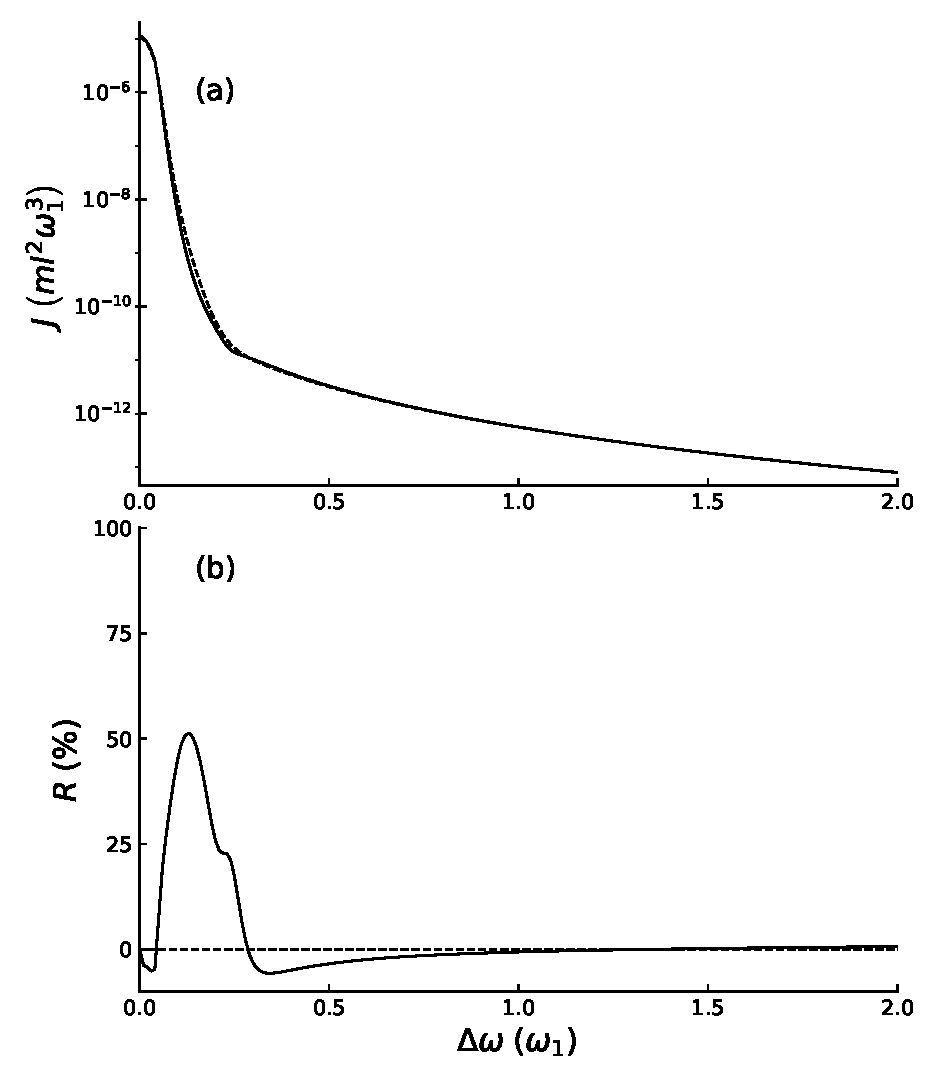
\includegraphics[width=\linewidth]{Figures/Graded_24Mg_FluxAndRectification_VS_FreqGradient.eps}
    \caption{Graded chain of $N=15$ $^{24}$Mg$^+$ ions. (a) Stationary fluxes for different frequency increments:
$J_\rightarrow$   (for $T_L = T_H$ and $T_R = T_C$, dashed line); $J_\leftarrow$ (for $T_L = T_C$ and $T_R = T_H$, solid line)
(b) Rectification factor. Parameters: $\omega_1 = 2 \pi \times 1$ MHz, $l = 5.25\;\mu$m, $a = 4.76\, l$ ($25\,\mu$m), $\delta_H = -0.02 \,\Gamma$, and $\delta_C = -0.1 \, \Gamma$.}
    \label{fig:RFG}
\end{figure}

To compare the results by solving Eq. \eqref{eq:Dynamics} and averaging and those from the algebraic method we  simulated a frequency graded chain with a trapping frequency $\omega_1 = 2\pi \times 50$ kHz for the leftmost ion, see Fig. \ref{fig:Temperature_Profiles_Magnesium}.  The number of ions interacting with the laser beams (three on each bath) is consistent with the lattice constant and typical waists of Gaussian laser beams \cite{Leupold2015,Lo2015}. To set the trap distance we fix first the characteristic length  $l =  \left(\frac{q^2}{4\pi\varepsilon_0}\frac{1}{m\omega_1^2}\right)^{1/3}$ as the distance for which the Coulomb repulsion of two ions equals the trap  potential energy for an ion at a distance
$l$ away from the center of its trap.
If $a<l$, the Coulomb repulsion of the ions is stronger than the trap confinement which makes the ions jump from their traps. With the parameters used in this section we have $l = 38.7\,\mu$m and set $a = 1.29 \,l=50\,\mu$m. The detunings of the \textit{hot} and \textit{cold} lasers are $\delta_H = -0.02 \, \Gamma$, and $\delta_C = -0.1 \, \Gamma$ which gives temperatures $T_H \approx 12$ mK and $T_C \approx 3$ mK. We fix the value $\Delta\omega = 0.5 \, \omega_1$ for the frequency increment.

The results of the two methods are in very good agreement. In the scale of Fig. \ref{fig:Temperature_Profiles_Magnesium} (a)
the calculated local temperatures are undistinguishable. In the calculation based on solving the dynamics we had to integrate Eq. \eqref{eq:Dynamics} for $N_{trials} = 1000$ realizations of white noise $\bm{\xi}(t)$. The method based on the system of moments
shortened the calculation time with respect to the dynamical trajectories   by a factor of $1/700$. In fact, the time gain is even more important because
the dynamical method requires further processing, performing a time averaging to compute the stationary flux in addition to noise averaging, see Fig.  \ref{fig:Temperature_Profiles_Magnesium} (b).


Additionally, the relaxation to the steady state slows down when the frequencies of the traps increase since the deterministic part of the Langevin equation dominates the dynamics over the stochastic part, entering an under-damped regime. In contrast, this increase does not affect the
algebraic method.
%%%%%%%%%%%%%%%%%%%%
\begin{figure}[t]
    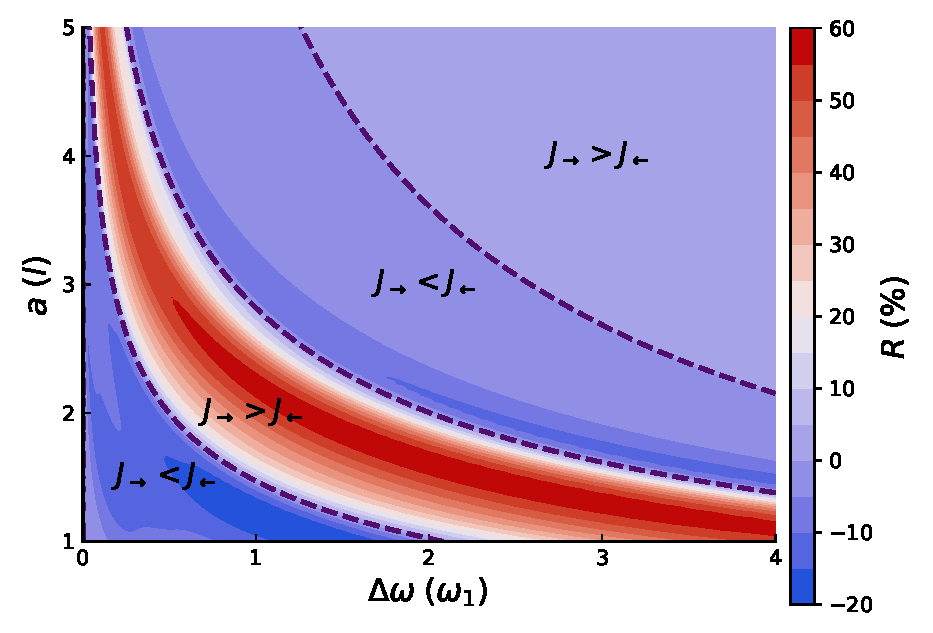
\includegraphics[width=\linewidth]{Figures/Graded_24Mg_Rectification_VS_Gradient_and_lattConstant.eps}
    \caption{ Rectification factor in a graded chain of $N=15$ $^{24}$Mg$^+$ ions for different trap distances and frequency increment. The dashed lines are for $R = 0$ and delimit the regions $J_\rightarrow > J_\leftarrow$ and $J_\rightarrow < J_\leftarrow$. The parameters  are $\omega_1 = 2 \pi \times 1$ MHz, $l = 5.25\,\mu$m, $\delta_H = -0.02 \,\Gamma$, and $\delta_C = -0.1 \, \Gamma$.}
    \label{fig:Graded_24Mg_Rectification_VS_Gradient_and_lattConstant}
\end{figure}
%
%
%
%
\subsection{Rectification in frequency graded chains \label{GradedChains}}
%
%
\begin{figure}
    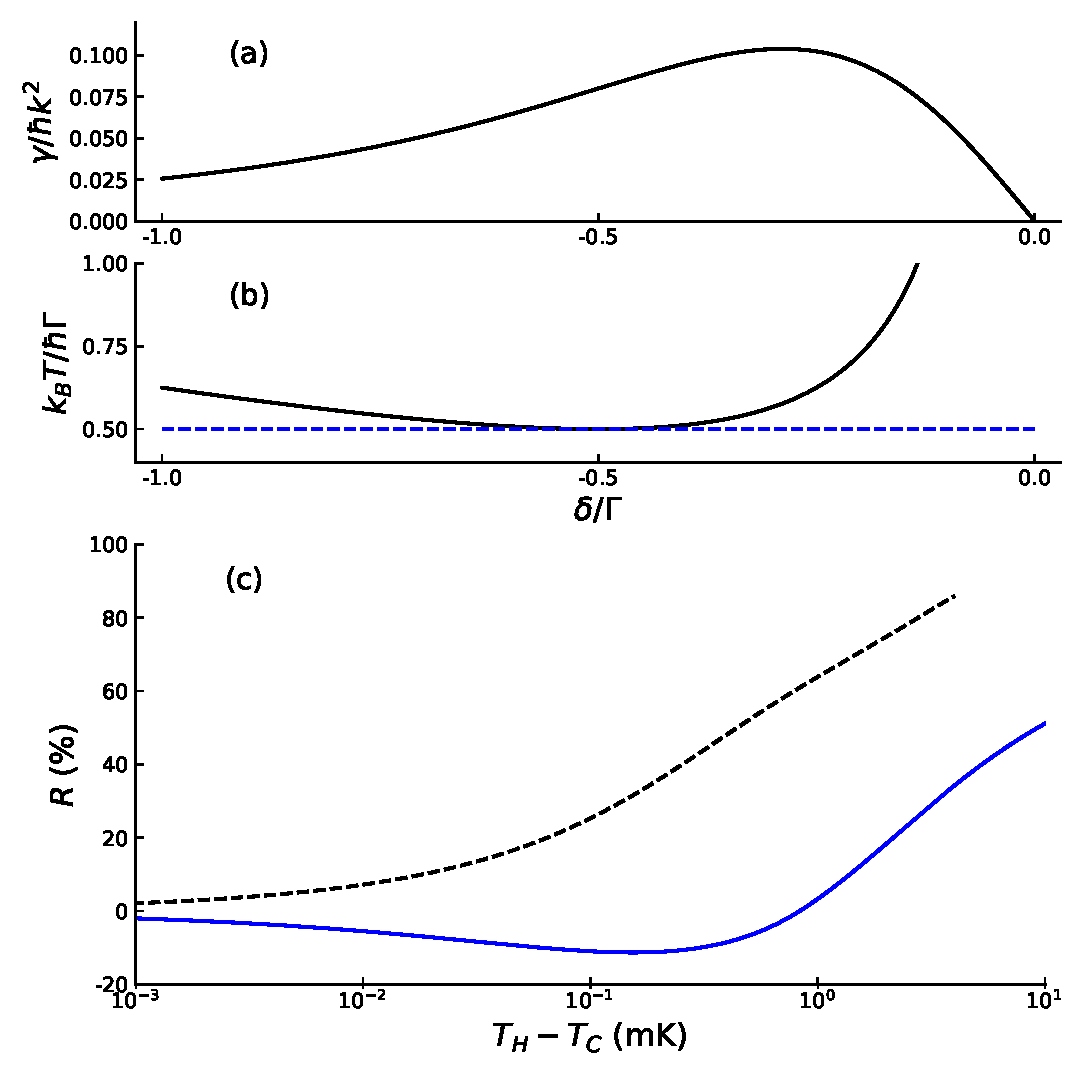
\includegraphics[width=\linewidth]{Figures/R_as_function_of_TemperatureBias.eps}
    \caption{ (a) Friction coefficient defined in Eq. \eqref{eq:DopplerCooling}. (b) Bath temperature defined in Eq. \eqref{eq:Doppler}. (c) Rectification as a function of the temperature difference between the hot and cold baths $T_H -T_C$ for $\delta_H$ below (dashed black line) and above (solid blue line) the Doppler limit, and $\delta_C=\delta_D$ (Doppler limit). Parameters: $\omega_1 = 2 \pi \times 1$ MHz, $\Delta \omega = 0.15 \, \omega_1$, $l = 5.25\,\mu$m, $a = 4.76 \, l$.}
    \label{fig:RD}
\end{figure}
%
In this subsection we demonstrate rectification for the frequency graded chain. We  used the method described in section \ref{steadyState} for $^{24}$Mg$^+$ ions with the same parameters for the baths used before. We fix the trapping frequency of the leftmost trap to $\omega_1 = 2\pi \times 1$ MHz, and a trap spacing $a = 4.76\, l$ ($25\,\mu$m) (the  characteristic length is $l = 5.25\,\mu$m). Figure \ref{fig:RFG} depicts  the results with these parameters in a graded chain. Figure \ref{fig:RFG} (a) shows that both
$J_\rightarrow$ and $J_\leftarrow$
% the right-going flux (dashed line) and the left-going flux (solid line)
decrease rapidly as the frequency increment  is increased.
%In Fig. \ref{fig:Graded_24Mg_FluxAndRectification_VS_FreqGradient} we see that
The rectification reaches its maximum value for a frequency difference of $\Delta\omega \approx 0.1 \omega_1$. The fluxes cross so there are some points where the rectification is exactly zero, besides the trivial one at $\Delta\omega = 0$, at $\Delta\omega = 0.05\,\omega_1,\;0.3\,\omega_1,\;1.3\,\omega_1$. At these points the direction of rectification reverses, presumably as a consequence of the changes in the match/mismatch of the temperature dependent local power spectra.
The change of rectification direction occurs for all the choices of parameters, as displayed in Fig. \ref{fig:Graded_24Mg_Rectification_VS_Gradient_and_lattConstant}. Figure \ref{fig:Graded_24Mg_Rectification_VS_Gradient_and_lattConstant} gives the rectification factor for different trap distances and frequency increments.  $0$-rectification curves separate regions with different rectification direction. The second region in Fig. \ref{fig:Graded_24Mg_Rectification_VS_Gradient_and_lattConstant} (starting from the left) would be the most interesting one to build a thermal diode, since rectification reaches its largest values there.

{For small values of $\Delta \omega$ there is little asymmetry in the chain and therefore modest rectification is expected whereas a very large $\Delta \omega$ implies very high trapping frequencies on the right implying too strong a
confinement and vanishing interactions. This bottleneck decreases the fluxes in both directions and  the rectification. However, since $\Delta \omega$ is controllable,
and the range of values of $\Delta \omega$ for which rectification is larger can be also controlled with the intertrap distance $a$, see Fig. \ref{fig:Graded_24Mg_Rectification_VS_Gradient_and_lattConstant},
the existence of a rectification window
does not imply a major limitation.}

\begin{figure}
    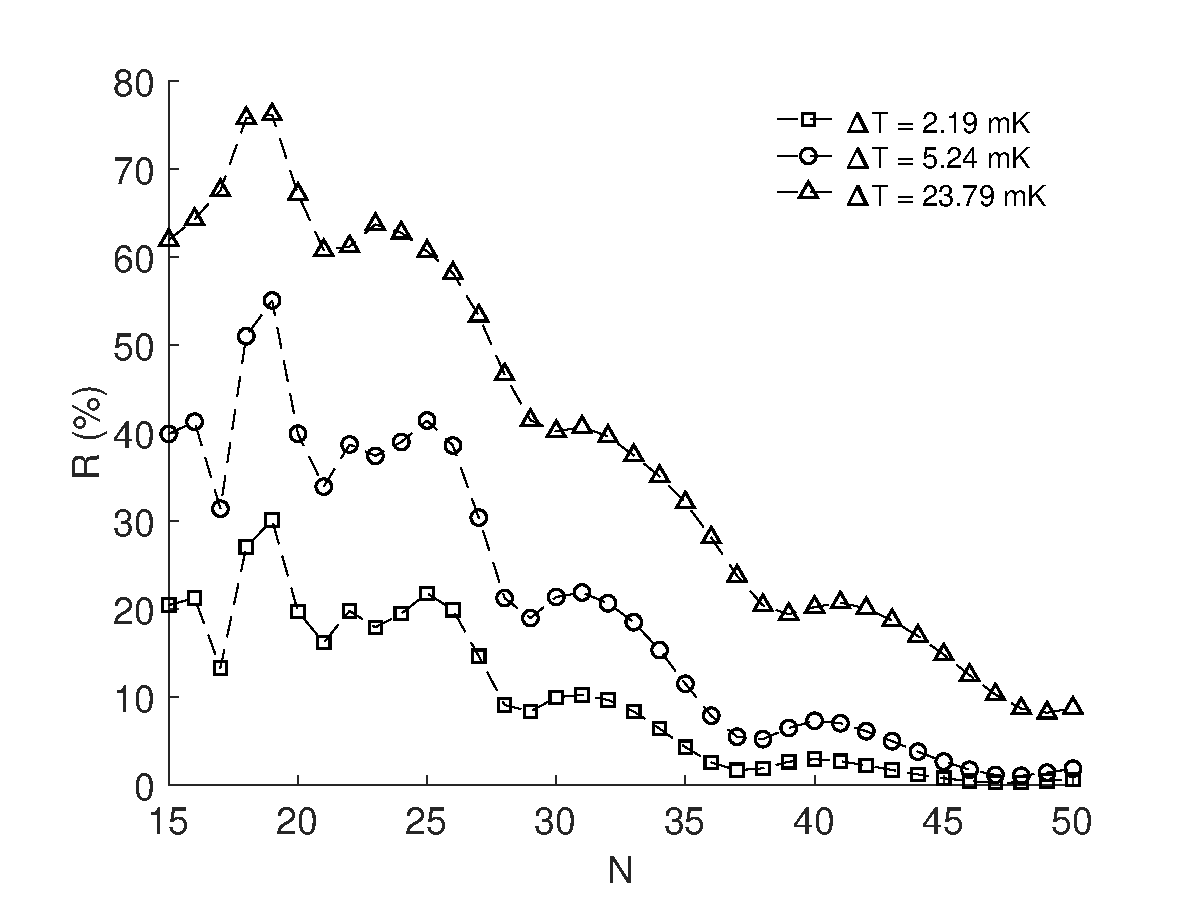
\includegraphics[width=\linewidth]{Figures/Changing_N.eps}
    \caption{Rectification factor for different bath temperature differences $\Delta T$ as the number of ions is increased. The detuning of the cold bath laser is set to the Doppler limit $\delta_C = - \Gamma / 2$. $\omega_1 = 2 \pi \times 1$ MHz, $\Delta \omega = 0.15 \, \omega_1$, $l = 5.25\,\mu$m, $a = 4.76 \, l$.}
    \label{fig:N_Dependence}
\end{figure}
%
%
\subsection{Same bath temperatures, different bath couplings\label{TC}}
%
%
As already mentioned below Eq. (\ref{eq:Doppler}), above and below the detuning  $\delta_D=-\Gamma/2$ corresponding to the  Doppler limit temperature, the optical molasses allow for
two different couplings (two pairs of friction and diffusion coefficients in Eq. (\ref{eq:DopplerCooling})) between the ions and the laser corresponding to the same bath temperature.
This duality may be seen explicitly in Fig. \ref{fig:RD}. Specifically Fig. \ref{fig:RD} (a) depicts the variation of the friction coefficient for values of $\delta$ around $\delta_R$,  and Fig. \ref{fig:RD} (b) the corresponding temperatures.
Interestingly, the different couplings imply different rectification factors.
% To check if this requirement is fulfilled we have calculated the rectification factor for different temperatures in the baths.
If we set $\delta_C = \delta_D=-\Gamma / 2$,  i.e., the cold bath is cooled to the Doppler limit, $\delta_H$ can be chosen to be below or above $\delta_D$ for the same temperature $T_H$. The corresponding rectification factors for the two choices
are shown in  Fig. \ref{fig:RD} (c),
%We see that it is possible to achieve comparable rectifications for smaller temperature differences when $\delta_H<\delta_D$.
%Note that since the effective laser temperatures depend on the linewidth $\Gamma$ of the atomic transition, the range of temperatures that can be reached is limited to the mK. Although other works have shown rectification in temperatures of the order of 100 K \cite{Elzouka2017}, the nature of the rectification mechanism and the physical system are very different. Here we have considered an atomic system, instead of a macroscopic one, where the temperatures are intrinsically low.
which
demonstrates that significant rectification can be achieved by choosing $\delta_H<\delta_D$ for temperature increments that
are smaller than or of the order of $T_C=T_D$, for example $R\approx 20\%$ for $\Delta T=0.1 T_C$, or $R\approx 60\%$
for $\Delta T= T_C$.  Finding good rectification at low (relative) temperature differences is considered to be one on the challenges
in asymmetric heat transport research \cite{Zhang2015}.


%. The temperature of the hot bath is controlled by changing the detuning of its laser. Any detuning we choose for the hot bath is going to give a larger temperature, since the cold one is already set to the minimum posible value at the Doppler limit. We can do this by setting a detuning below ($\delta_H < -\Gamma / 2$) or above ($\delta_H > -\Gamma / 2$) the Doppler limit for the hot bath, see Fig. \ref{fig:RD} (b). The dynamics of the chain will be different for the same temperature bias depending if the detuning of the hot bath is below or above the Doppler limit because the corresponding friction coefficients will be different, see Fig. \ref{fig:RD} (a). As a consequence, different currents and rectifications will be found in the chain depending if $\delta_H$ is below or above the Doppler limit. In Fig. \ref{fig:RFG} maximum rectification values are around $60 \,\%$ with temperature differences of around 10 mK. This temperature difference is roughly four times the temperature of the cold bath, so it is a relatively high temperature difference. Thus, in principle, it looks that high temperature differences are needed to obtain rectification. However, this is not always the case.
%
%
%
\subsection{Dependence with ion number\label{IN}}
%
Keeping in mind that scaling the frequency-graded ion chain  to a large numbers of ions is not a realistic option in this setting,
it is nevertheless important to
study the dependence with ion number from small to moderate numbers.  In Fig. \ref{fig:N_Dependence} we observe an overall trend in which the rectification decreases with the number of ions in the chain (while it increases with temperature bias $\Delta T$ in the studied range). This effect is easy to understand, as increasing $N$
while keeping the total variation of the trapping frequency $\Delta \omega$ constant, the frequency gradient  decreases. This
lowers  the  asymmetry in the chain and the rectification factor. Oscillations with $N$ superimposed to the global trend are more visible at the smaller $N$ values giving  an optimal $N$ value at $N=19$.

\subsection{Graded versus segmented\label{GS}}
%
We have also compared the performance of the graded thermal diode and a segmented version in which the left half of the chain is trapped with frequency $\omega_1$ and the right half (including the middle ion) with $\omega_1+\Delta \omega$. Even though the optimal rectification  in Fig. \ref{fig:GS} (a)  for the segmented chain is larger than for the graded chain, the fact that the fluxes are generally much larger for the graded chain, see Fig. \ref{fig:GS} (b), makes the graded chain more interesting for applications.



\begin{figure}[t]
    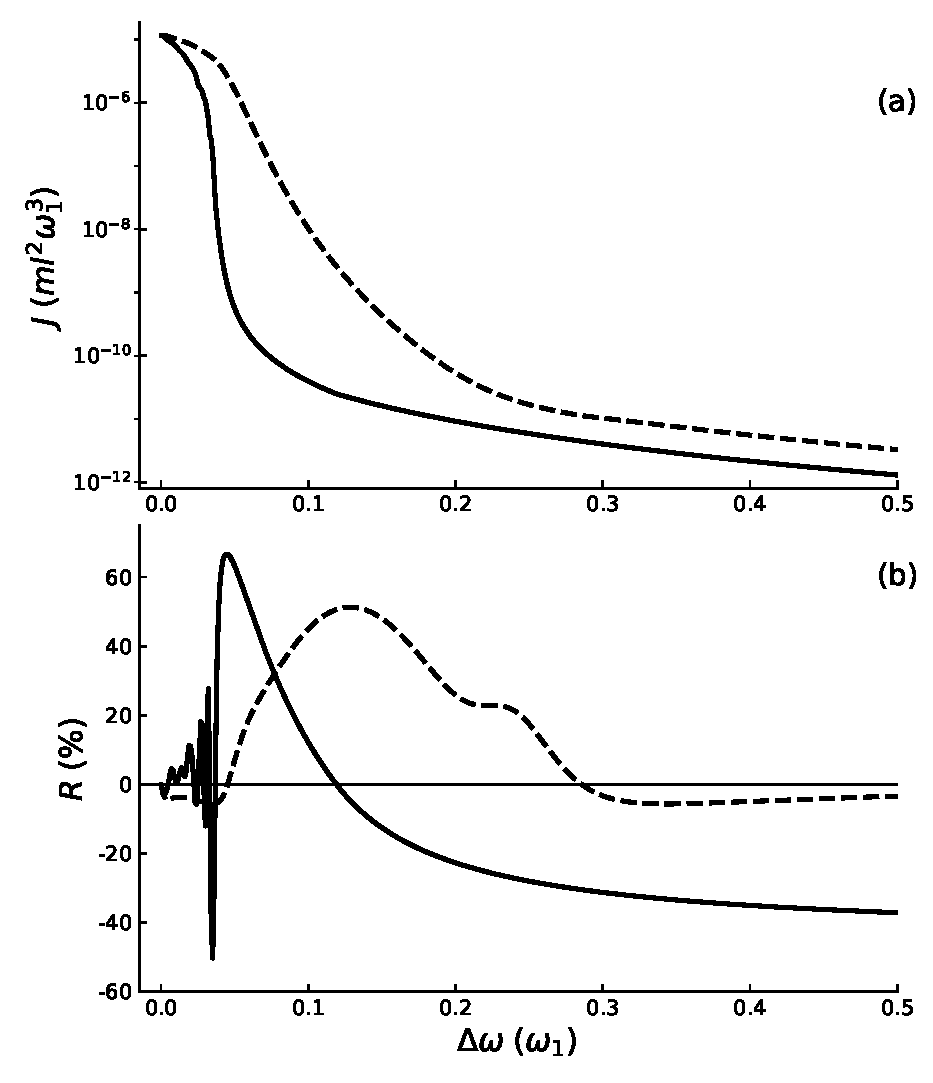
\includegraphics[width=\linewidth]{Figures/24Mg_Comparacion_Graded_AND_Segmented.eps}
    \caption{Comparison of graded and segmented chains with $N=15$ $^{24}$Mg$^+$ ions. (a) Maximum
    of $J_\rightarrow$ and $J_\leftarrow$
     for the graded and segmented chain for different frequency increments. (b) Rectification factor: graded chain (dashed lines); segmented chain (solid lines). Parameters: $\omega_1 = 2 \pi \times 1$ MHz, $l = 5.25\,\mu$m, $a = 4.76 \, l$, $\delta_H = -0.02 \, \Gamma$, and $\delta_C = -0.1 \, \Gamma$.}
    \label{fig:GS}
\end{figure}





\begin{figure}[t]
    \includegraphics[width=\linewidth]{Figures/fig_lambda_centered.eps}
    \caption{Thermal conductivity through the chain for $T_L > T_R$ (empty squares), and $T_L < T_R$ (filled triangles). $\omega_1 = 2 \pi \times 1$ MHz, $\Delta \omega = 0.15 \, \omega_1$, $l = 5.25\,\mu$m, $a = 4.76 \, l$, $\delta_H = -0.02 \,\Gamma$ and $\delta_C = -0.1 \, \Gamma$.}
    \label{fig:Thermal_conductivity}
\end{figure}
%
%
\section{Summary and discussion\label{ConclusionsRectificationChainOfIons}}
%
%
%
%
In this article we have numerically demonstrated heat rectification in a chain of ions trapped in individual microtraps with graded frequencies, connected at both ends to thermal baths
created by optical molasses. An alternative to implement a graded
frequency profile in the lab
could be combining a collective Paul trap for all the ions with on-site dipolar laser forces \cite{Freitas2015,Enderlein2012,Bermudez2013,Schneider2010}.

A goal of this article is to connect two communities, ion trappers and
researchers on heat-rectification models. The results found are encouraging and demonstrate the potential of a trapped-ion platform to experimentally investigate heat rectification schemes. Trapped ions are quite interesting to this end because  they are highly controllable,  and may easily adopt several features to enhance rectification, such as
the ones explored here (long-range interactions and an asymmetrical gradation),
or others such as time dependent forces \cite{Li2012,Riera-Campeny2018}, or different nonlinearities in onsite forces.
The limitations and application domain should also be clear,  the proposed platform is circumscribed to cold temperatures of the order of hundreds of $\mu$K to mK achieved by Doppler cooling.
In this sense it is not aimed at competing  with (it is rather complementary to)
proposals for which experiments  \cite{Chang2006,Leitner2013,Kobayashi2009,Elzouka2017} or simulations \cite{Zhang2015,Ma2018,Reid2019}
demonstrate thermal rectification
at room temperature or for hundreds of K.
Also, the number of ions should realistically be kept small so the proposed ion chain
is not aimed at achieving a macroscopic diode length, but at playing a role in thermal diode research
and in the context of ion-trapped based quantum technologies.

Methodologically, the calculation of the steady state has been performed with an algebraic approach much faster than
the time-consuming integration and averaging over noise and time of the dynamical equations.
The algebraic approach linearizes the forces around equilibrium positions which, in this system and for the realistic parameters considered  is well justified and tested numerically.
The results found provide additional evidence that simple linear models may  rectify heat flow \cite{Pereira2017}.  We  underline that our linear
model is, arguably,  even simpler than some linear ``minimalist, toy models'' in \cite{Pereira2017} that showed rectification (our on-site forces are already linear from the start and the temperature dependence of explicit model parameters is only in the coefficients of the Langevin baths), with the important bonus of being also realistic.

To shed some more light on the mechanism behind the observed rectification we may analyze the local thermal conductivities
$\lambda[x,T(x)]$
{defined in a continuous model by} \cite{Peyrard2006}
%
\begin{equation}
    J = \lambda [x,T(x)]\left|\frac{dT (x)}{dx}\right|,
    \label{eq:thermalConductivityDefinition}
\end{equation}
%
where $J$ is the stationary heat current and $T(x)$ the local temperature.
(We use the modulus of the temperature derivative for consistency with our (positive) definition of $J$.)
In our model we discretize the coordinate with the ion index
and the temperature derivative is discretized as
%
\begin{equation}
    \frac{dT_n}{dx} = \frac{T_{n+1}-T_{n-1}}{x^{eq}_{n+1}-x^{eq}_{n-1}}.
    \label{eq:finiteDifferences}
\end{equation}
%
%
%\blue{In an article of Peyrard \cite{Peyrard2006} the performance of a segmented rectification is studied and the rectification mechanism is understood by means of a thermal conductivity that is both temperature and position dependent. This thermal conductivity is derived from assuming that the heat current follows the Fourier law locally
Through integration, it is clear that when $\lambda$ depends on both temperature and position rectification is possible.
In the continuous model the temperature increment between the  baths is
%
\begin{equation}
|T_L-T_R|=\int_0^L  \frac{J}{\lambda[x,T(x)]} dx
\end{equation}
%
so that the key for rectification is a different integral of the inverse of the  conductivities in the two scenarios ($T_L=T_H, T_R=T_C$  with conductivity $\lambda_\rightarrow[x,T_\rightarrow(x)]$ along a local temperature decreasing from the left
or the reversed one, $T_R=T_H, T_L=T_C$ with conductivity $\lambda_\leftarrow[x,T_\leftarrow(x)]$ along an increasing local temperature.
Particularly favorable for rectification is the scenario where one of the lambdas is above the other one for all $x$.
Figure \ref{fig:Thermal_conductivity} shows that this is essentially the case in our model, at least along the most relevant part of the integral.
